%%% LaTeX Template: Two column assignment for BRSU
%%% Based on two column article from: http://www.howtotex.com/
%%% Preamble
\documentclass[	DIV=calc,%
				paper=a4,%
				fontsize=11pt,%
				twocolumn]{scrartcl}	 % KOMA-article class

\usepackage{lipsum}	% Package to create dummy text
\usepackage{blindtext}
\usepackage[english]{babel}	                          % English language/hyphenation
\usepackage[protrusion=true,expansion=true]{microtype} % Better typography
\usepackage{amsmath,amsfonts,amsthm}					 % Math packages
\usepackage{graphicx}	                          % Enable pdflatex
\usepackage[svgnames]{xcolor}	                          % Enabling colors by their 'svgnames'
\usepackage[hang, small,labelfont=bf,up,textfont=it,up]{caption} % Custom captions under/above floats
\usepackage{epstopdf}	 % Converts .eps to .pdf
%\usepackage{subfig}	     % Subfigures
\usepackage{booktabs}	 % Nicer tables
\usepackage{fix-cm}       % Custom fontsizes
\usepackage{listings}
\usepackage{soul}
\usepackage{float}
\usepackage{url}
\usepackage{amsmath}
\usepackage{caption}
\usepackage{subcaption}
%\usepackage[hyperref = true, backend=biber, style=numeric, sorting = none]{biblatex}

%%% Custom sectioning (sectsty package)
\usepackage{sectsty}	 % Custom sectioning (see below)
\allsectionsfont{%% Change font of al section commands
	\usefont{OT1}{phv}{b}{n}%% bch-b-n: CharterBT-Bold font
	}

\sectionfont{%% Change font of \section command
	\usefont{OT1}{phv}{b}{n}%% bch-b-n: CharterBT-Bold font
	}


\definecolor{brsugrey}{rgb}{0.9, 0.9, 0.9}
\definecolor{brsublue}{rgb}{0, 0.594, 0.949}


\newcommand{\upperRomannumeral}[1]{\uppercase\expandafter{\romannumeral#1}}

%%% Headers and footers
\usepackage{fancyhdr} % Needed to define custom headers/footers
	\pagestyle{fancy} % Enabling the custom headers/footers
\usepackage{lastpage}	

% Header (empty)
\lhead{}
\chead{}
\rhead{}
% Footer (you may change this to your own needs)
\lfoot{\footnotesize 
\texttt{LAA} % Set to the course abbreviation 
\textbullet ~ Schoebel, Arriaga, Koripalli % Set to your name
\textbullet ~ Project Report \upperRomannumeral{1}} % Set the assignment number
\cfoot{}
\rfoot{\footnotesize page \thepage\ of \pageref{LastPage}}	% "Page 1 of 2"
\renewcommand{\headrulewidth}{0.0pt}
\renewcommand{\footrulewidth}{0.4pt}



%%% Creating an initial of the very first character of the content
\usepackage{lettrine}
\newcommand{\initial}[1]{%
     \lettrine[lines=3,lhang=0.3,nindent=0em]{
     				\color{brsublue}
     				{\textsf{#1}}}{}}

%%% Title, author and date metadata
\usepackage{titling}	% For custom titles

\newcommand{\HorRule}{\color{brsublue}% Creating a horizontal rule
					 \rule{\linewidth}{1pt}%
					 \color{black}
					 }

\pretitle{\vspace{-30pt} \begin{flushleft} \HorRule 
				\fontsize{25}{25} \usefont{OT1}{phv}{b}{n} \color{gray} \selectfont 
				}
\title{Learning and Adaptivity Report:
\\Convolutional Neural Networks and Sparse Coding for Image Classification of RoboCup@Home and RoboCup@Work Objects}% Title of your article goes here
\posttitle{\par\end{flushleft}\vskip 0.5em}

\preauthor{\begin{flushleft}
\large \lineskip 0.25em \usefont{OT1}{phv}{b}{sl} \color{brsublue}}
\author{Octavio Arriaga, Nitish Koripalli, Maximilian Schoebel   }	% Author name goes here
\postauthor{\footnotesize \usefont{OT1}{phv}{m}{sl} \color{Black} 
BRS University of Applied Sciences % Institution of author
\\email:
\\octavio.arriaga@smail.inf.h-brs.de
\\maximilian.schoebel@smail.inf.h-brs.de
\\nitish.koripalli@smail.inf.h-brs.de
\par\end{flushleft}\HorRule}

\date{\today} 

%%% Begin document
\begin{document}
\maketitle
\thispagestyle{fancy} % Enabling the custom headers/footers for the first page 
% The first character should be within \initial{}
\initial{O}\textbf{bject recognition is an actively researched field in machine learning. Two underlying approaches that can be used for robust object recognition algorithms are hierarchical and sparse feature extraction. In this work we explore convolutional neural networks and sparse coding which embody these properties respectively. We test their object recognition performance in a structured and industrial environment: RoboCup@Work and Robocup@Home.}

\section{Introduction}

\subsection*{Convolutional Neural Networks}

Deep learning techniques yield state-of-the-art results for object detection and recognition; specifically Convolutional Neural Networks (CNNs) have proven to be extremely useful for image classification. Therefore, we introduce our own deep architecture model, and train it to classify objects from the RoboCup-@Home competition.

In order to understand the CNN used for our training example, first we would have to define the discrete convolution operator for 2-Dimensions. 

\begin{equation}
S(i,j) = (I * k)(i,j) = \sum_m \sum_n I(m,n)K(i-m,j-n)
\end{equation}

This equations can be thought of as performing an discrete-operation to all possible values of an input I. This can also be seen as the application of a filter to an image-Matrix I, see Figure \ref{2d_cnn}.

\begin{figure}[H]
    \centering
    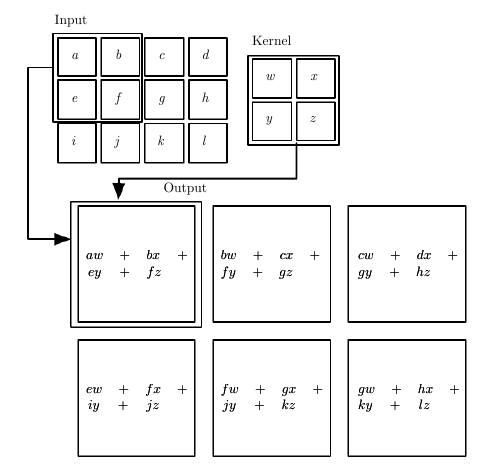
\includegraphics[width=.9\linewidth]{data/2d_cnn.png}
    \caption{Discrete convolution applied to an input-matrix \cite{Goodfellow-et-al-2016-Book}}
    \label{2d_cnn}
\end{figure}

The input-matrix can represent an image, and the output is a matrix-like multiplication to a section of the input image which is the size of the kernel. This operation is repeated for all possible input values of the image.

In the typical CNN network terminology, the first argument is often refered to as the \textit{input}, the second argument is the \textit{kernel}, and the output by applying the convolution, is the \textit{feature map}.

As can be seen in Figure \ref{2d_cnn}, each output pixel results from applying the kernel to a small patch of the input image. These patches do overlap however and do can be bigger then in Figure \ref{2d_cnn}. Several kernels are trained and applied to the input image and thereby form the first convolutional layer.

The general Convolutional Network architecture consists of several convolutional layers stacked over each other, each of them followed by a pooling layer. Pooling layers perform, depending on their kind, a combination of a small output patch of the previous convolutional layer. Following figure \ref{max_pooling} shows a simple example of max-pooling, where only the maximum value of the convolutional layer's output is passed on as the output of the pooling patch.

\begin{figure}[H]
    \centering
    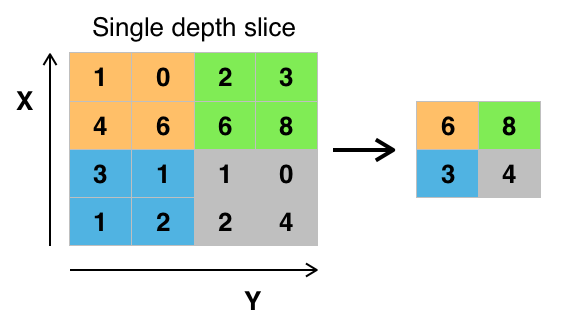
\includegraphics[width=.9\linewidth]{data/max_pooling.png}
    \caption{Max-pooling \cite{pooling_cnn}}
    \label{max_pooling}
\end{figure}

The outputs of the pooling layers form a filtered, lower-dimensional representation of the previous convolutional layer. By stacking pairs of convolutional- and pooling layers, the representations get more abstract with each layer and since each convolution and pooling operation reduces the dimensionality, the upper layers operate on a bigger scope of the input image.

The use of pooling-layers also makes the learned lower-level representations, i.e. features, invariant to small shifts in position. The reduction of dimensionality in depth with each layer is also called subsampling.

The following figure \ref{typical_architecture} shows the typical architecture of a Convolutional Neural Network.

\begin{figure}[H]
    \centering
    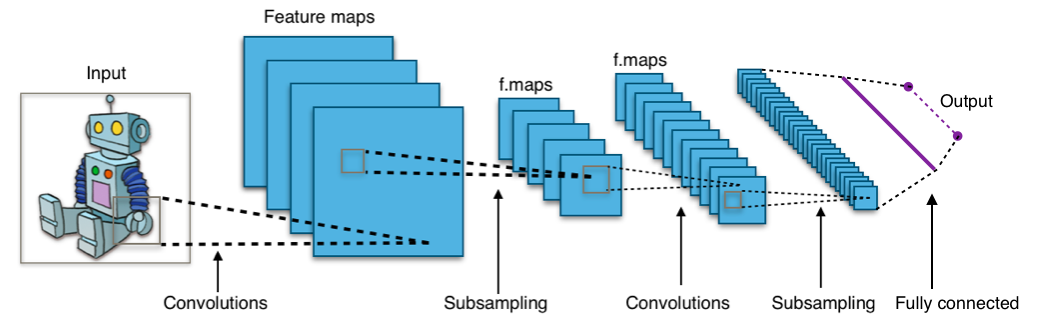
\includegraphics[width=\linewidth]{data/typical_cnn.png}
    \caption{Typical CNN architecture \cite{pooling_cnn}}
    \label{typical_architecture}
\end{figure}

After training several layers of convolution and subsampling (e.g. pooling) learned a fixed size and abstract representation of the input image. The last subsampling layer is then followed by several fully connected layers which act as a classifier to distinguish the image-classes present in the dataset. The complete architecture is then trained end-to-end (including the fully connected layers).

\subsection*{Intermediate CNN Results and Visualization}

Before performing any training on our data, we wanted to test the capabilities of the used framework \textit{Keras} \cite{keras_page} on a well tested dataset. Therefore we trained a smaller model with 2D convolutional layers and max-pooling using the MNIST \cite{mnist} dataset (see Figure \ref{cnn_results_2}). In Figure \ref{cnn_results_3} we show the results after the first convolutional layer. This model was trained using the Keras framework on top of Theano.

\begin{figure}[H]
    \centering
    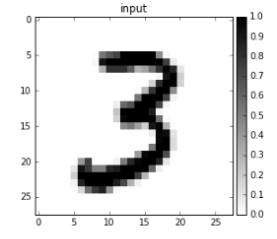
\includegraphics[width=0.8\linewidth]{data/cnn_results_2.png}
    \caption{Image taken from MNIST dataset. Every row and column represents one pixel size.}
    \label{cnn_results_2}
\end{figure}

The learned 32 kernels after the convolutional layer can be seen in the following image. 

\begin{figure}[H]
    \centering
    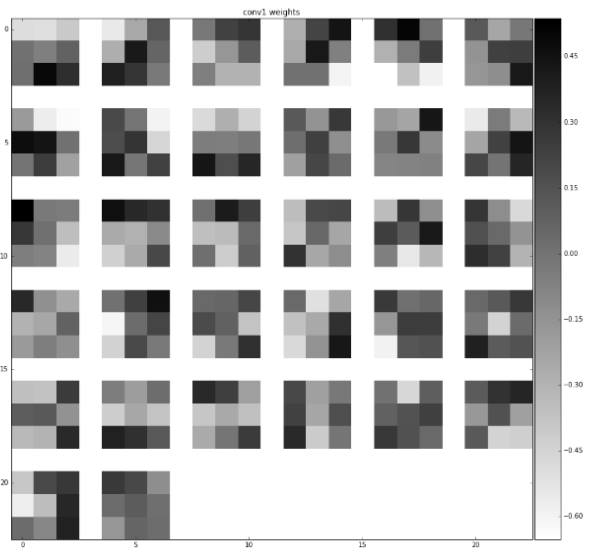
\includegraphics[width=0.8\linewidth]{data/cnn_results_3.png}
    \caption{All 32 kernels learned from the first convolutional layer.}
    \label{cnn_results_3}
\end{figure}

And the application of these filters or learned kernels to the image presented in Figure \ref{cnn_results_2} is shown below. 

\begin{figure}[H]
    \centering
    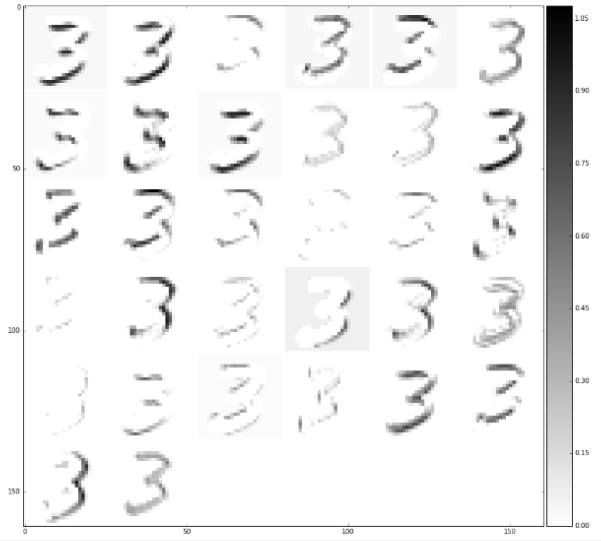
\includegraphics[width=0.8\linewidth]{data/cnn_results_4.png}
    \caption{All 32 Kernels applied to an example of the datase.}
    \label{cnn_results_4.png}
\end{figure}

We can observe that just after the first convolution layer, the model is able to distinguish the shape of the contours of the data. 

\subsection*{Sparse Coding}
Sparse coding is a class of unsupervised methods for learning sets of over-complete bases to represent data efficiently. The aim of sparse coding is to find a set of basis vectors $\phi_{i}$ such that we can represent an input vector $\mathbf{x}$ as a linear combination of these basis vectors. \cite{ufldl_sparse_coding}

$$ \mathbf{x} = \sum_{i=1}^{k} \alpha_{i}\phi_{i} $$

While techniques such as Principal Component Analysis (PCA) allow us to learn a complete set of basis vectors efficiently, we wish to learn an over-complete set of basis vectors to represent input vectors $\mathbf{x}\in\mathbb{R}^n$ (i.e. such that k $>$ n). The advantage of having an over-complete basis is that our basis vectors are better able to capture structures and patterns inherent in the input data. However, with an over-complete basis, the coefficients $\alpha_{i}$ are no longer uniquely determined by the input vector $\mathbf{x}$. Therefore, in sparse coding, we introduce the additional criterion of \textbf{sparsity} to resolve the degeneracy introduced by over-completeness.

\begin{figure}[H]
    \centering
    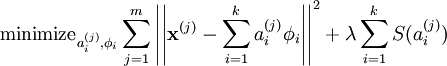
\includegraphics[width=0.8\linewidth]{data/sc_data/sc_equation.png}
    \caption{The cost function used for finding the basis functions and the coefficients $\alpha$.}
    \label{cnn_results_4.png}
\end{figure}

S(.) is a sparsity cost function which penalizes ai for being far from zero. We can interpret the first term of the sparse coding objective as a reconstruction term which tries to force the algorithm to provide a good representation of $\mathbf{x}$ and the second term as a sparsity penalty which forces our representation of $\mathbf{x}$ to be sparse. The constant $\lambda$ is a scaling constant to determine the relative importance of these two contributions. The intuition for sparse coding can be seen as the following \cite{olshausen_1997} :

\textit{cost\_function = reconstruction\_error + sparseness} 

\noindent The equation minimizes the cost function in an iterative manner. For one iteration, first the encoding (the extraction of coefficients $\alpha$) is kept constant and a dictionary $\phi$ that minimizes the cost function is found and then keeping the dictionary contant the encoding (the extraction of coefficients $\alpha$) that minimizes the cost function is found.


\subsection*{Intermediate Sparse Coding Results and Visualization}
We wanted to test the framework for sparse coding which is \textit{sparsex} \cite{sparsex}. We trained a 400 dimension dictionary on 40000 images of Yann LeCun's MNIST database \cite{mnist}. Each image is 28x28 pixels. We obtained a result of 89.9  $\pm$ 0.5 \% accuracy. The visualizations of the data preprocessing, feature extraction and results are shown:

\begin{figure}[H]
    \centering
    
\includegraphics[width=0.3\linewidth]{data/sc_data/sc_mnist_image.jpg}
    \caption{Image taken from MNIST dataset. Every row and column represents one pixel size. The image size is 28x28 pixels.}
    \label{sc_mnist_image}
\end{figure}


\begin{figure}[H]
    \centering
    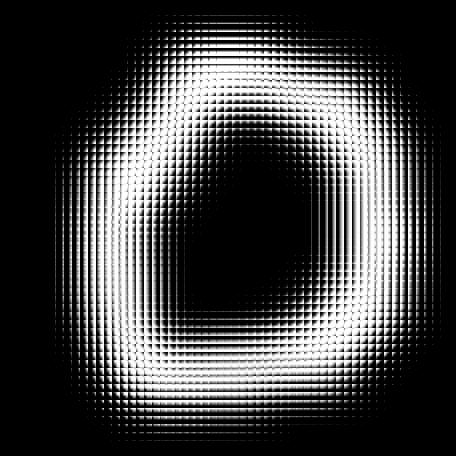
\includegraphics[width=0.45\linewidth]{data/sc_data/sc_mnist_patches_montage.jpg}
    \caption{A montage of 8x8 pixel patches extracted from the original 28x28 image. A total of 441 patches are extracted per image.}
    \label{sc_mnist_patches_montage}
\end{figure}


\begin{figure}[H]
    \centering
    
\includegraphics[width=0.45\linewidth]{data/sc_data/sc_mnist_whitened_patches_montage.jpg}
    \caption{A montage of whitened patches which is a result of applying whitening or sphering to the patches obtained in figure 9.}
    \label{sc_mnist_whitened_patches_montage}
\end{figure}
 
 
\begin{figure}[H]
    \centering
    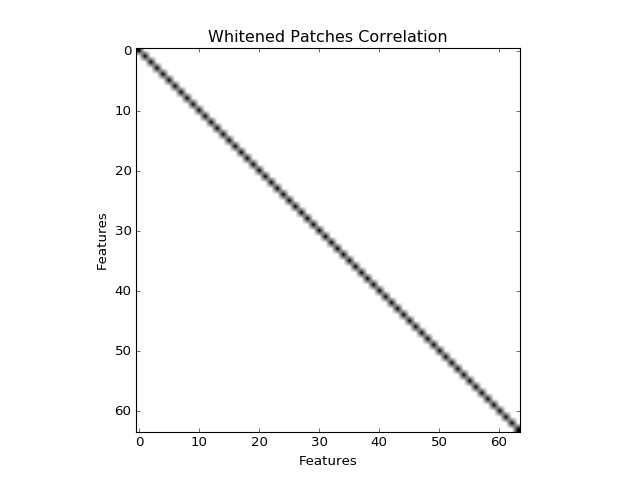
\includegraphics[width=0.8\linewidth]{data/sc_data/sc_mnist_whitened_patches_correlation.png}
    \caption{A correlation plot of the whitened patches which shows decorrelation (reduced redundancy) within the data since the features are correlated only with themselves.}
    \label{sc_mnist_whitened_patches_correlation}
\end{figure}

\begin{figure}[H]
    \centering
    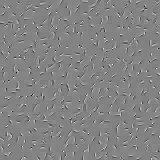
\includegraphics[width=0.7\linewidth]{data/sc_data/sc_mnist_dictionary.jpg}
    \caption{A montage of the trained dictionary which has 400 elements (20x20) where each element has a dimension of 8x8 pixels. The dictionary elements are similar to the gabor filters.}
    \label{sc_mnist_dictionary}
\end{figure}

\begin{figure}[H]
    \centering
    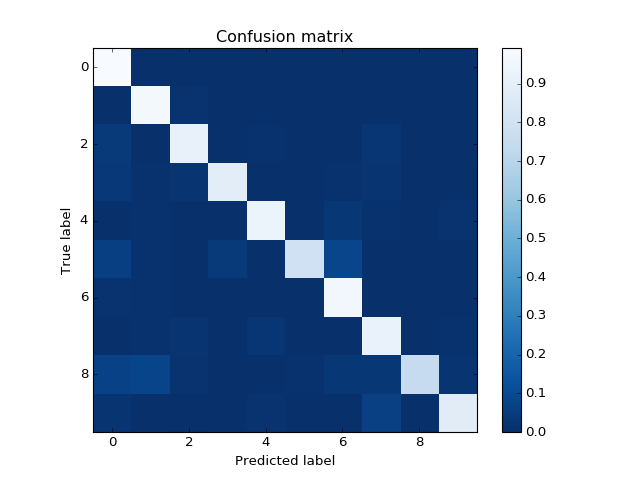
\includegraphics[width=1.0\linewidth]{data/sc_data/sc_mnist_confusion_matrix.png}
    \caption{A confusion matrix of the results to show how the classifier confuses one class label with another. From the figure it is clear that the classifier is confident about each class due to the prominent diagonal.}
    \label{sc_mnist_confusion_matrix}
\end{figure}

\section{Approach}

\subsection*{CNN-Architecture}
Our final model consists of 4 convolutional layers, each followed by a max-pooling layer. The first layer takes 32x32 pixels for each color channel (RGB) as inputs, resulting in 3*32*32 input units.
After the final max-pooling layer a two layered fully connected network is added as classifier. The final layer uses softmax-activation function, each previous layer uses rectified linear units.

\subsection*{CNN-Training}
The model was trained using stochastic gradient descent with a learning-rate of $0.01$, weight-decay of $10^{-6}$ and momentum of 0.9 for 100 epochs.
Dropout is used in every layer to reduce overfitting.

The training dataset was splitted into a training-set (80\%) and a testing-set (20\%).

\subsection*{Sparse Coding}
The general approach we used for sparse coding involves the following steps. Each step has its respective citation that describes the implementation and motivation behind that step.
\begin{enumerate}
\item Splitting data into training and test set
	\begin{enumerate}
	\item 5-fold cross validation \cite{sklearn_cross_validation}
	\end{enumerate}
\item Preprocessing
	\begin{enumerate}
	\item Image resizing \cite{coates2011analysis}
	\item Patch extraction \cite{coates2011analysis}
	\item Patch normalization \cite{coates2011analysis}
	\item Patch whitening \cite{coates2011analysis}
	\end{enumerate}
\item Feature extraction
	\begin{enumerate}
	\item Dictionary learning \cite{mairal2009online, spams}
	\item Sparse encoding \cite{mairal2009online, spams}
	\item Sparse encoding sign-split 
	\item Max-pooling  \cite{yang2009linear, scherer2010evaluation}
	\end{enumerate}
\item Classification
	\begin{enumerate}
	\item Standardization of features \cite{wiki_feature_scaling}
	\item Training linear SVM classifier using training data \cite{svm_light}
	\item Classifying the test data \cite{svm_light}
	\end{enumerate}
\end{enumerate}

First we split the dataset into training and test sets using 5 fold cross validation. For one experiment we resized the images to 67x67 pixels and extracted 8x8 pixel patches from the images with a stride of 1. We then applied preprocessing techniques like normalization or feature scaling to make the pixel values of the patches be in an appropriate range and applied whitening to decorrelate the patches. We then use the training set patches to learn a dictionary of 625 elements. We use a subsampled set of patches for learning the dictionary because it is a time consuming process and also since many patches repeat themselves in the dataset we do not have a lot of loss of information. Using the learnt dictionary we encode the patches into a sparse weighted sum of basis functions (dictionary elements), which is the feature extraction phase. We then reduce the dimensionality of the data using max pooling. Finally we concatenate the pooled patch encodings of one image into one long feature vector for that image. This feature vector, depending on the pool filter size may have a dimensionality between 5000-32000. We then pass this feature vector as input to the SVM linear classifier for training. We repeat the process above for the test data and obtain predictions from the classifier.


\section{Datasets}
\subsection*{@Home Objects}
For training the final model we collected a datset consisting of a total of 424 Images of the following RoboCup@Home-Objects:
\begin{enumerate}
    \setlength\itemsep{-0.25em}
    \item Pack of Coffee
    \item Paper coffee-cup
    \item Juice-box
    \item Big ketchup bottle
    \item Small ketchup bottle
    \item Mr Muscle cleaner
    \item Pepper
    \item Pringles can
    \item Water bottle
\end{enumerate}


\subsection*{@Work Objects}
For training the final model we collected a datset consisting of a total of 360 Images of the following RoboCup@Work-Objects \cite{robocup_atwork_rulebook}:
\begin{enumerate}
    \setlength\itemsep{-0.25em}
	\item F20 20 B
	\item F20 20 G
	\item S40 40 B 
	\item S40 40 G
	\item M20 100 
	\item M20 
	\item M30
	\item R20
	\item Bearing Box
	\item Bearing
	\item Axis
	\item Distance Tube 
	\item Motor 
\end{enumerate}

The pictures were taken with a low resolution camera (640x480 pixel) equivalently to the camera mounted on Jenny-COB, from a fixed angle and on a fixed background (white table).
The Images were then cropped and scaled to fit the network input size of 32x32 pixels for @Home objects and 67x67 pixels for @Work objects.

\section{Results}

\subsection*{CNN}
After 100 epochs of training, which took approximately 5 minutes and 47 seconds, the model achieved an accuracy 98.55\%. The model has additionally been tested on the dataset that was created from the RoboCup@Work objects and yielded an accuracy of 83.48\%.

We took a cluttered picture by accident, our model was able to classify the object correctly.

\begin{figure}[H]
    \centering
    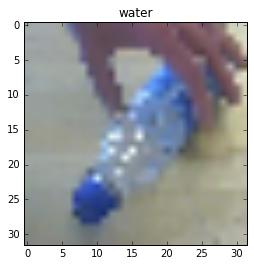
\includegraphics[width=0.5\linewidth]{data/cluttered_image}
    \caption{Cluttered image of the class "Water bottle" with hand of experimenter. The network was able to classify the image correctly.}
\end{figure}

Our datasets, as well as the implementation of the CNN is available here: \begin{small}\url{https://github.com/oarriaga/machine_learning_algorithms/tree/master/algorithms/convolutional_neural_network}\end{small}

When plotting the activations of convolutional layers, the abstraction and reduction in dimensionality that occurs can be made visible.

\begin{figure}[H]
    \centering
    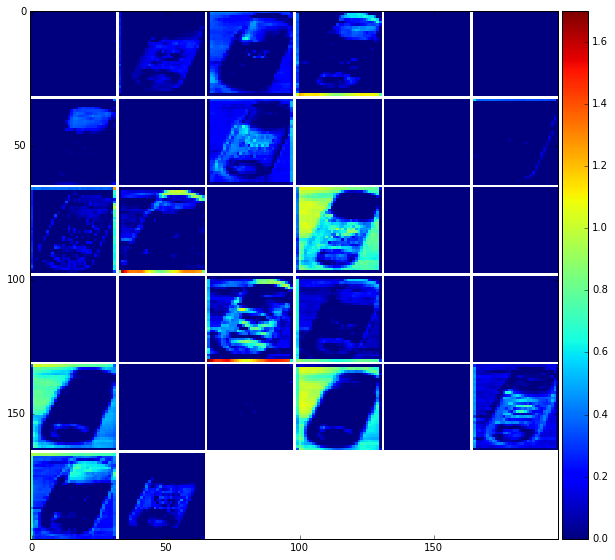
\includegraphics[width=0.5\linewidth]{data/final_cnn_firstlayer}
    \caption{Output after the first convolutional layer of our network, when presented with an input image.}
\end{figure}

\begin{figure}[H]
    \centering
    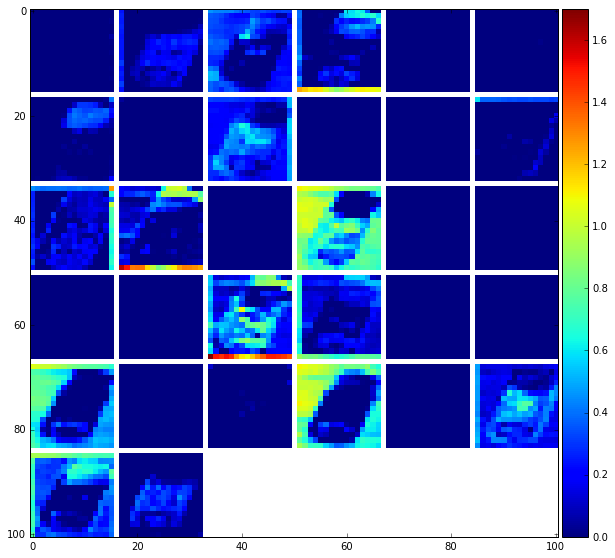
\includegraphics[width=0.5\linewidth]{data/final_cnn_secondlayer}
    \caption{Output after the second convolutional layer of our network, when presented with an input image.}
\end{figure}

\begin{figure}[H]
    \centering
    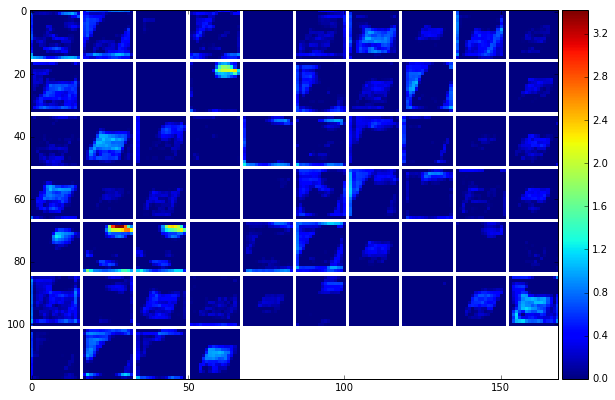
\includegraphics[width=0.5\linewidth]{data/final_cnn_thirdlayer}
    \caption{Output after the third convolutional layer of our network, when presented with an input image.}
\end{figure}

\begin{figure}[H]
    \centering
    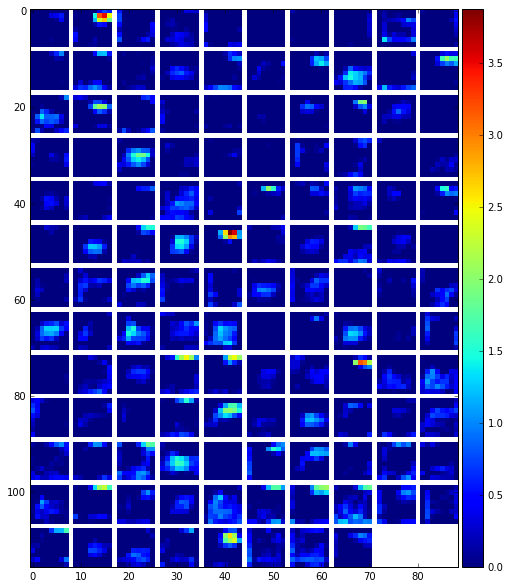
\includegraphics[width=0.5\linewidth]{data/final_cnn_fourthlayer}
    \caption{Output after the fourth convolutional layer of our network, when presented with an input image.}
\end{figure}

The following two images show final representations that our model learned. It can be seen that the representations look very similar, but are different in a specific area. The corresponding pictures are indeed the same object, but rotated in the picture. The differing areas therefore correspond to the roatation of the object.

\begin{figure}[H]
    \centering
    \begin{subfigure}[b]{0.45\linewidth}
        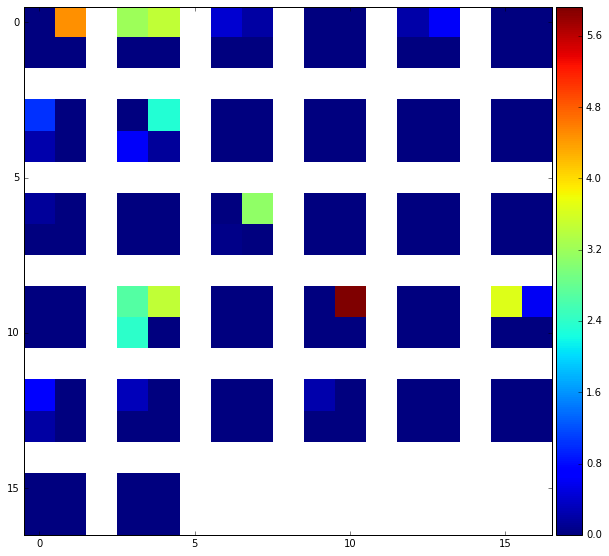
\includegraphics[width=\linewidth]{data/final_1.png}
    \end{subfigure}
    \hfill
    \begin{subfigure}[b]{0.45\linewidth}
        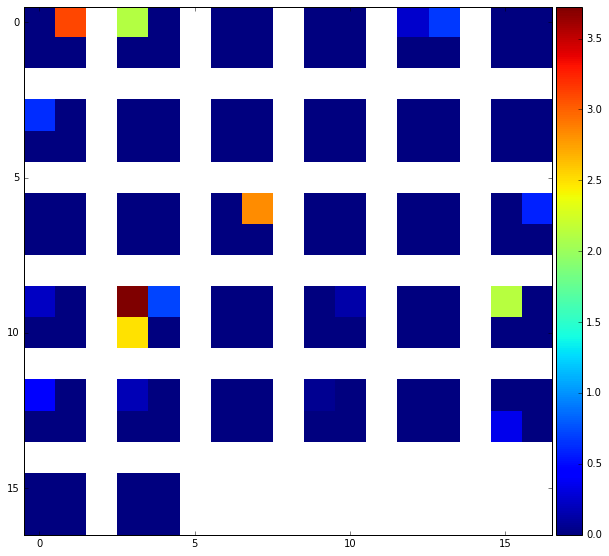
\includegraphics[width=\linewidth]{data/final_2.png}
    \end{subfigure}
    \caption{Final Representations for two ketchup-bottles, which are rotated.}
    \label{}
\end{figure}

\begin{figure}[H]
    \centering
    \begin{subfigure}[b]{0.45\linewidth}
        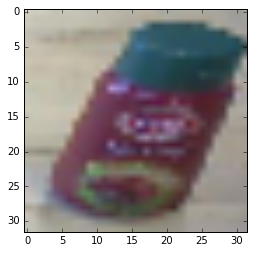
\includegraphics[width=\linewidth]{data/ketchup_final_1.png}
    \end{subfigure}
    \hfill
    \begin{subfigure}[b]{0.45\linewidth}
        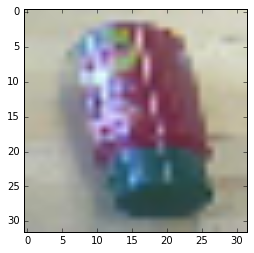
\includegraphics[width=\linewidth]{data/ketchup_final_2.png}
    \end{subfigure}
    \caption{The two images of rotated ketchup bottles.}
    \label{}
\end{figure}


\subsection*{Sparse Coding}
After tests on 5-fold cross validation, we were able to achieve 71.63 \% accuracy. Following are some of the visualizations from the experiments:

\begin{figure}[H]
    \centering
    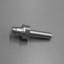
\includegraphics[width=0.3\linewidth]{data/sc_data/sc_atwork_image.jpg}
    \caption{Image taken from @Work dataset. Every row and column represents one pixel size. The image size is 67x67 pixels.}
    \label{sc_atwork_image}
\end{figure}


\begin{figure}[H]
    \centering
    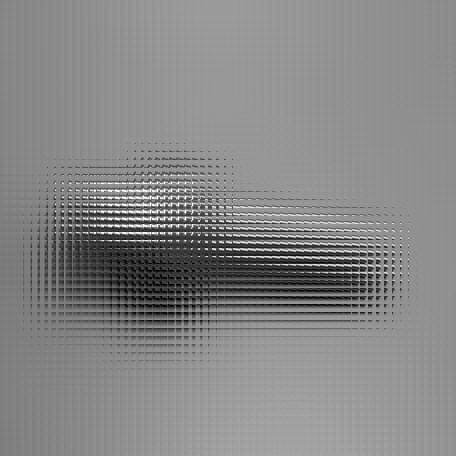
\includegraphics[width=0.6\linewidth]{data/sc_data/sc_atwork_patches_montage.jpg}
    \caption{A montage of 8x8 pixel patches extracted from the original 67x67 image. A total of 3600 patches are extracted per image.}
    \label{sc_atwork_patches_montage}
\end{figure}


\begin{figure}[H]
    \centering
    
\includegraphics[width=0.6\linewidth]{data/sc_data/sc_atwork_whitened_patches_montage.jpg}
    \caption{A montage of whitened patches which is a result of applying whitening or sphering to the patches obtained in the previous figure.}
    \label{sc_atwork_whitened_patches_montage}
\end{figure}
 
 
\begin{figure}[H]
    \centering
    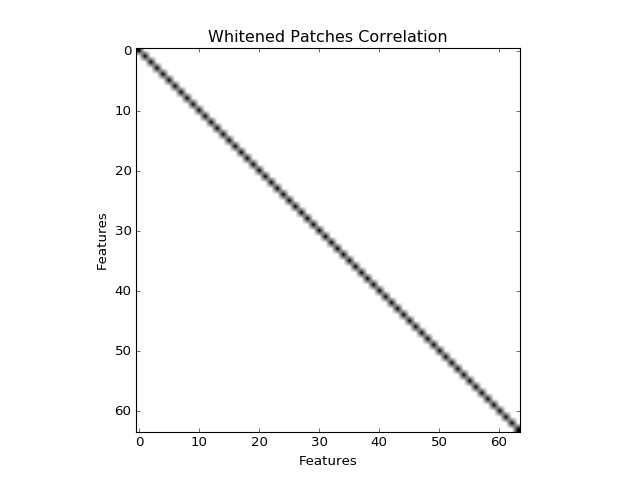
\includegraphics[width=0.7\linewidth]{data/sc_data/sc_atwork_whitened_patches_correlation.png}
    \caption{A correlation plot of the whitened patches which shows decorrelation (reduced redundancy) within the data since the features are correlated only with themselves. This is a correct and expected behaviour.}
    \label{sc_atwork_whitened_patches_correlation}
\end{figure}

\begin{figure}[H]
    \centering
    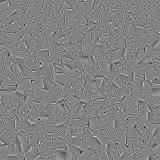
\includegraphics[width=0.5\linewidth]{data/sc_data/sc_atwork_dictionary.jpg}
    \caption{A montage of the trained dictionary which has 400 elements (20x20) where each element has a dimension of 8x8 pixels. The filters that have been learnt here are not ideal and have a lot of noise  as compared to the filters shown for the MNIST dataset in a previous figure.}
    \label{sc_atwork_dictionary}
\end{figure}

\begin{figure}[H]
    \centering
    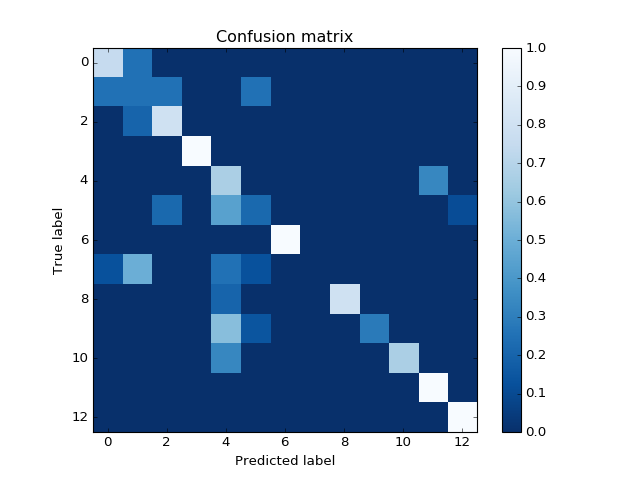
\includegraphics[width=0.8\linewidth]{data/sc_data/sc_atwork_confusion_matrix.png}
    \caption{A confusion matrix of the test vs predicted results which shows no results for label 7 which is object R20. Also we can see a lot of confusion among class labels 0, 1, 2, 4 and 5.}
    \label{sc_atwork_confusion_matrix}
\end{figure}

The implementation of the Sparse Coding is available here: \begin{small}\url{https://github.com/nitred/sparsex}\end{small}

\section{Conclusion}

\section*{CNN}
We implemented and trained a CNN on a dataset that we created from RoboCup@Home and RoboCup@Work objects. The results were very good, a real system could easily function with a classification accuracy of 98.55\%. The accuracy for RoboCup@Work objects is: 83.48\%.

In the future several issues should be addressed however. Since the dataset we created was relatively small, overfitting might be an issue. A second dataset could be created with the same objects but differnt conditions as lighting, background, occlusions and viewing angle. Artificial methods for enlarging the dataset, like applying small transformations could also be used.

\section*{Sparse Coding}
We implemented and trained a feature extraction using Sparse Coding and classification using SVMs on a dataset that we created from RoboCup@Work objects. The results were insufficient to be used for the Robocup competitions with 71.83 \% accuracy.

For the future there are several problems that can be solved. Firstly, the cropping of the images was done manually which caused scaling errors which may have made some objects look like others. Secondly, the \textit{sparsex} implementation currently only supports grayscale images and should support RGB images which would add additional features. Thirdly, the dictionary that was learnt on the training data had a lot of noise in it, therefore in the future the right parameters for dictionary learning must be explored. Lastly, we need to collect a larger dataset so as to extract more meaningful features and have enough data to properly train the classifier.

\onecolumn

\begin{thebibliography}{9}

\bibitem{ufldl_sparse_coding}
    \url{http://ufldl.stanford.edu/wiki/index.php/Sparse\_Codingst}

\bibitem{sparsex}
    \url{https://github.com/nitred/sparsex}

\bibitem{olshausen_1997}
Olshausen, Bruno A., and David J. Field. \textit{"Sparse coding with an overcomplete basis set: A strategy employed by V1?."} Vision research 37.23 (1997): 3311-3325.

\bibitem{mnist}
    \url{http://yann.lecun.com/exdb/mnist/}

\bibitem{coates2011analysis}
Coates, Adam, Andrew Y. Ng, and Honglak Lee. "An analysis of single-layer networks in unsupervised feature learning." International conference on artificial intelligence and statistics. 2011.

\bibitem{mairal2009online}
Mairal, Julien, et al. "Online dictionary learning for sparse coding." Proceedings of the 26th annual international conference on machine learning. ACM, 2009.

\bibitem{spams}
    \url{http://spams-devel.gforge.inria.fr/}

\bibitem{svm_light}
    \url{http://svmlight.joachims.org/}

\bibitem{yang2009linear}
Yang, Jianchao, et al. "Linear spatial pyramid matching using sparse coding for image classification." Computer Vision and Pattern Recognition, 2009. CVPR 2009. IEEE Conference on. IEEE, 2009.

\bibitem{scherer2010evaluation}
Scherer, Dominik, Andreas Müller, and Sven Behnke. "Evaluation of pooling operations in convolutional architectures for object recognition." Artificial Neural Networks–ICANN 2010. Springer Berlin Heidelberg, 2010. 92-101.

\bibitem{sklearn_cross_validation}
    \url{http://scikit-learn.org/stable/modules/generated/sklearn.cross\_validation.StratifiedKFold.html}

\bibitem{wiki_feature_scaling}
    \url{https://en.wikipedia.org/wiki/Feature\_scaling}

\bibitem{robocup_atwork_rulebook}
    \url{http://www.robocupatwork.org/rules.html}

\bibitem{Goodfellow-et-al-2016-Book}
Ian Goodfellow Yoshua Bengio and Aaron Courville, \textit{Deep Learning}, 2016, Book in preparation for MIT Press. \url{www.deeplearning.org}

\bibitem{pooling_cnn}
Wikipedia-article "Convolutional Neural Networks" \url{https://en.wikipedia.org/wiki/Convolutional_neural_network}

\bibitem{keras_page}
Keras: Deep Learning library for Theano and TensorFlow \url{www.keras.io}

\end{thebibliography}

\HorRule

\end{document}
